

\chapter{الگوهای طراحی اعمال شده}
({\color{red} بهنگام‌سازی شد: اعمال بازخورد })

\newpage
\section{Factory}
این الگو زمانی استفاده می‌شود که قصد داریم بدون اینکه به استفاده‌کننده اعلام کنیم چگونه یک شئ را می‌سازیم، شئ را ساخته و به وی تحویل دهیم. ما از این الگو در کلاس AccessLevel استفاده کرده‌ایم. استفاده به این صورت است که یک کلاس انتزاعی
\LTRfootnote{abstract}
 به نام AccessLevel داریم که سه زیرکلاس آن را پیاده‌سازی می‌کنند. هر کدام از این سه کلاس، نمایانگر یک نوع از سطح دسترسی هستند. حال یک AccessLevelFactory داریم که با توجه به کاربر،‌ و از طریق تابع getAccessLevel() یک AccessLevel تحویل استفاده‌کننده می‌دهد.\\
 به جای این الگو، شاید به نظر برسد الگوهای Creational دیگری چون 
 \lr{Abstract Factory}
  قابل اعمال باشد. در حالی که چنین نیست. الگوی
 \lr{Abstract Factory}
 در نقش واسطی است که به استفاده‌کننده اجازه می‌دهد از طریق یک Factory خاص، یک Product خاص تحویل بگیرد که در زمانی کاربرد دارد که چند Factory داشته باشیم. حال آنکه در مورد استفاده‌ی ما، تنها یک Factory موجود است.
در شکل 
\ref{f200}
کلاس طراحی حاصل از اعمال این الگو قابل مشاهده است. در این شکل، کلاس  AccessLevelFactory
وظیفه‌ی ساختن شئ را بر عهده دارد. مشتری  برای ساختن شئ از  یکی از زیرکلاس‌های AccessLevel درخواست را به AccessLevel نمی‌دهد. بلکه آن را برعهده‌ی AccessLevelFactory می‌گذارد و با تابع getAaccessLevel() شئ ساخته شده را دریافت می‌کند. جهت تاکید، کلاس AccessLevel  که AccessLevelFactory
با آن در  ارتباط است، از نوع abstract است. 

\begin{figure}[H]
	\centering
	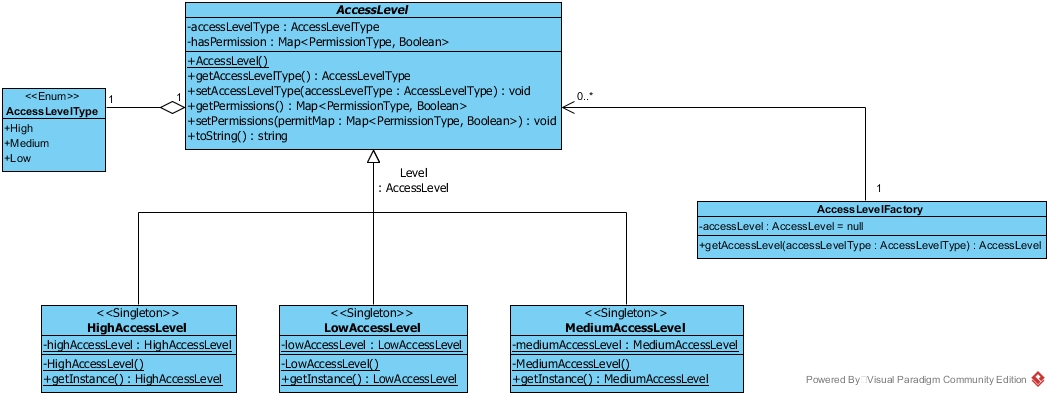
\includegraphics[scale=0.5]{img/pattern/factory}
	\caption{استفاده از الگوی Factory}
	\label{f200}
\end{figure}

\newpage
\section{Singleton}
این الگو زمانی استفاده می‌شود که دقیقا یک نمونه از یک کلاس لازم باشد. کلاس‌های Catalogue که در لایه‌ی منطق قرار دارند و همچنین کلاس‌های DAO که در لایه‌ی ارتباط با پایگاه‌داده قرار دارند، همگی از این الگو پیروی می‌کنند. این الگو، در مقابل استفاده از متد‌های ایستا در اینگونه کلاس‌ها استفاده شده است. چرا که استفاده از کلاس در طراحی شئ‌گرا تنها به عنوان قالب قابل قبول است؛ و نه به عنوان یک موجودیت که به طور مستقل کاری انجام می‌دهد.

\begin{figure}[H]
	\centering
	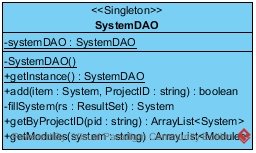
\includegraphics[scale=0.5]{img/pattern/singleton1}
	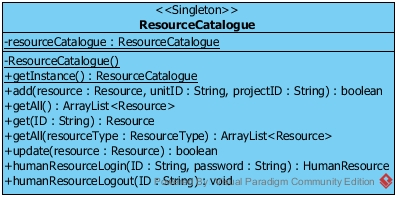
\includegraphics[scale=0.5]{img/pattern/singleton2}
	\caption{دو مورد استفاده از الگوی Singleton}
	\label{f201}
\end{figure}

برای استفاده از این الگو، ابتدا سازنده
\LTRfootnote{Constructor}
را به صورت خصوصی
\LTRfootnote{Private}
در می‌آوریم. سپس یک فیلد ایستا  از نوع کلاس و به صورت خصوصی ایجاد می‌کنیم. حال کدی که برای آن می‌نویسیم، چنین خواهد بود:
\begin{latin}
\begin{lstlisting}[language=java]
public static ClassName getInstance() {
	if (className == null)
		className = new ClassName();
	return className;
}
\end{lstlisting}
\end{latin}
در شکل
\ref{f201}
دو نمونه از کاربرد این الگو در پروژه‌ی حاضر قابل مشاهده است.

\newpage
\section{Observer}
این الگو زمانی استفاده می‌شود که تغییر در یک شئ، لازم است به اطلاع اشیای دیگری برسد. ما از این الگو در واسط کاربری استفاده کرده‌ایم. این سناریو را در نظر بگیرید: یک پنجره  A پروژه‌های موجود در سازمان را نشان می‌دهد. حال پنجره‌ی دیگری باز می‌شود تا در آن بتوان یک پروژه‌ی جدید اضافه کرد. پس از افزوده شدن پروژه جدید، باید بلافاصله در پنجره A پروژه‌ی جدید هم نمایش داده شود. هر هنگام که چنین سناریویی پیش می‌آید، از الگوی Observer استفاده می‌نماییم. (به عنوان نمونه‌ی دقیق‌تر، در کلاس‌های EditProject و ViewProjects) در مواردی که محتویاتی که لازم است روی صفحه نمایش داده شود زیاد است، با update کردن تنها بخش تغییر یافته را بهنگام‌سازی می‌کنیم و در نتیجه سرعت نیز بالا می‌رود.


\begin{figure}[H]
	\centering
	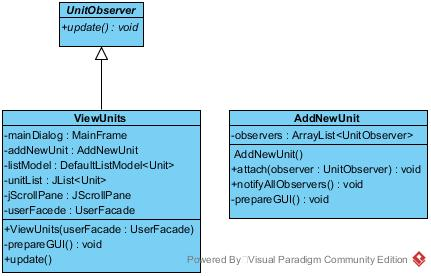
\includegraphics[scale=0.5]{img/pattern/observer}
	\caption{  استفاده از الگوی Observer}
	\label{f202}
\end{figure}

همان‌طور که به عنوان نمونه در شکل
\ref{f202}
قابل مشاهده است، یک واسط
\LTRfootnote{Interface}
به نام UnitObserver برای رصد کردن اضافه شدن واحد (از طریق کلاس AddNewUnit) ایجاد شده است. کلاسی که به دانستن این تغییر نیازمند است، کلاس ViewUnits است. در نتیجه واسط UnitObserver را پیاده‌سازی می‌کند؛ به عبارت دیگر، تابع update() آن را پیاده‌سازی می‌کند. در این تابع همه‌ی تغییراتی که با تغییر در AddNewUnit رخ می‌دهد انجام می‌شود. در کلاس AddNewUnit که تغییرات آن مد نظر بوده، تابعی با نام attach() ، notifyAllObservers() و  آرایه‌ای از UnitObserver وجود دارد. هنگامی  که یک UnitObserver  جدید به وجود می‌آید، خود با تابع attach() خود را آرایه‌ی موجود در AddNewUnit اضافه می‌کند. هرگاه تغییری توسط AddNewUnit به وجود آید، تابع notifyAllObservers() را صدا می‌زند تا تغییر به اطلاع همه‌ی Observer هایش برسد؛ به این صورت که تابع update() را در همه‌ی آن‌ها صدا می‌کند.


\newpage
\section{Façade}
این الگو زمانی استفاده می‌شود که بخواهیم یک واسط یکپارچه برای چند واسط سیستم ایجاد کنیم. بر روی لایه‌ی منطق، سه Façade تعریف شده است که عبارتند از: OperationFacade ،‌ UserFacade و ProjectFacade . هرکدام از این سه، واسط بخشی از کلاس‌های لایه‌ی منطق هستند. لایه‌ی نمایش، که شامل JFrame‌ ها و JDialog ها است، هیچ ارتباط مستقیمی با کلاس‌های لایه‌ی منطق ندارد. به عبارت دیگر، این سه Façade تعریف شده، واسطی بین لایه‌ی منطق و لایه‌ی نمایش محسوب می‌گردد. هر کدام از Façade ها، با تعدادی از کلاس‌های منطق در ارتباط هستند.\\
به طور دقیق‌تر، نقش هریک از  Façade ها عبارت است از:
\begin{itemize}
\item
کلاس OperationFacade ، با کلاس‌های مربوط به منابع در ارتباط است و امکانات مربوط به دریافت و بهنگام‌سازی منابع را بر عهده دارد.
\item
کلاس ProjectFacade ، با کلاس‌های مربوط به پروژه (و در نتیجه سیستم و ماژول) در ارتباط است و امکانات مربوط به دریافت و بهنگام‌سازی این موارد را بر عهده دارد.
\item
کلاس UserFacade ، موارد کاربری را بر عهده دارد؛ به این صورت که از طریق آن، ورود و خروج کاربران انجام می‌شود.
\end{itemize}

در شکل 
\ref{f203}
ProjectFacade
به همراه چند نمونه از کلاس‌های که از آن استفاده می‌کنند آورده شده است.  البته این کلاس طراحی کامل نیست و تنها به عنوان یک نمونه‌ و برای نمایش شمای کلی آورده شده است. کلاس‌های لایه‌ی نمایش (بالای شکل) به جای ارتباط مستقیم با کلاس‌های لایه‌ی منطق (پایین شکل) از طریق یک Façade (وسط شکل) به صورت غیرمستقیم ارتباط برقرار می‌کنند. همان‌طور که مشاهده می‌شود، با استفاده از  Façade در واقع یک مولفه
\LTRfootnote{Component}
 ساخته‌ایم. جزییات کلاس‌های آورده شده در شکل، در نمودار کلاس‌های طراحی قابل مشاهده است.

\begin{figure}[H]
	\centering
	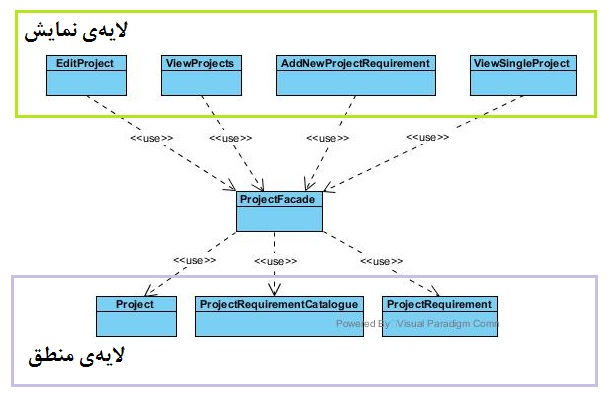
\includegraphics[scale=0.6]{img/pattern/facade}
	\caption{  استفاده از الگوی Façade}
	\label{f203}
\end{figure}
